\documentclass{article}
\usepackage[utf8]{inputenc}
\usepackage[spanish]{babel}
\usepackage{amsthm}
\usepackage{amsmath}
\usepackage{tipa}
\usepackage{graphicx}
\usepackage{hyperref}

\title{Una demostración del teorema de Kuratowski}
\author{Recopilada por Marcelo Lynch}
\date{Julio de 2015}

\newtheorem{lemma}{Lema}
\newtheorem{theorem}{Teorema}
\newtheorem*{definition}{Definicion}
\newtheorem*{obs}{Observación}
\newtheorem*{corollary}{Corolario}
\newtheorem*{notacion}{Notación}

\usepackage[margin=1.4in]{geometry}




\begin{document}

\maketitle

\section*{Introducción}
Se pretende en el siguiente documento demostrar de la manera más elemental posible el teorema de Kuratowski, que provee condiciones necesarias y suficientes para la planaridad de un grafo. \\ \\La demostración que se exhibe a continuación utiliza teoría elemental de grafos excepto en una ocasión, donde se utiliza el concepto de proyección estereográfica para demostrar (se deja el esquema de dicha demostración) un hecho que de todas maneras resulta intuitivo. Se enuncian el teorema de Euler y sus colorarios sin demostración. \\ \\ Existen demostraciones de naturaleza más topológica y geométrica que pueden resultar menos verbosas, pero la que aquí se presenta resulta especialmente interesante por revelar de manera bastante explícita y constructiva la subyacencia inevitable de $K_5$ y $K_{3,3}$ en los grafos no planos (en definitiva, lo que afirma el teorema).



\section*{Notación}
En lo que sigue, para un grafo $G$ notaremos el conjunto de vértices de $G$ con $V_G$, el conjunto de aristas de G con $E_G$, la conexidad por vértices de $G$ como $K_v(G)$. Para un vértice $v$, $g(v)$ denota el grado de v. $R_\infty$ denota la región externa de un grafo en una inmersión plana.

\section*{Consideraciones preliminares}

\begin{lemma}
Sea $G$ un grafo plano, y $e \in E_G$. Existe una inmersion plana tal que $e$ es frontera de $R_\infty$
\end{lemma}
 
\begin{proof}[Esquema de demostración]
Consideremos una inmersión plana de $G$. Si tiene a $e$ como frontera de $R_\infty$, no hay nada que demostrar. De lo contrario, basta considerar la inmersión plana sobre la superficie de una esfera (vía el mapeo inverso de la proyección estereográfica\footnote{Proyección estereográfica: \url{https://en.wikipedia.org/wiki/Stereographic_projection}}): una nueva proyección estereográfica sobre el plano con el polo norte en un punto de la región limitada por $e$, que resultará en la región externa en la proyección, con $e$ limitando $R_\infty$
\end{proof}

\begin{theorem}[Euler]
Sea $G$ conexo y plano. Si $v = \#V_G, e =  \#E_G$ y $r$ es el número de regiones en una inmersión plana de $G$, entonces $v - e + r = 2$
\end{theorem}

\begin{corollary}
Si $G$ es simple, sin lazos, conexo y plano, con $\#V_G \ge 3$, entonces $\#E_G \le 3\#V_G - 6$.
\end{corollary}

\begin{corollary}
Si $G$ es simple, conexo, bipartito y plano con $\#V_G \ge 3$, entonces $\#E_G \le 2\#V_G - 4$.
\end{corollary}

\begin{lemma}
$K_{3,3}$ y $K_5$ no son planos.
\end{lemma}

\begin{proof}[Demostración]
Inmediato a partir de los corolarios.

\end{proof}


\begin{definition}[Contracción de una arista]
Sea $G$ grafo, $e = \{u,v\} \in E_G$. La contracción de $e$ es una operación que da como resultado el grafo     $C_e(G) = (V', E')$, con
\begin{gather*}
    V' = (V_G \setminus \{u, v\}) \cup \{w\}, con \ w \notin V_G\\
    E' = E_G \setminus \{\{x,u\},\{x,v\} \in E_G\} \cup \{\{w,x\} / \{x,u\} \in E_G \vee \{x,v\} \in E_G\}
\end{gather*}
Es decir, fusiona los vértices $u$ y $v$ extremos de la arista $e$ en un solo vértice $w$, que será adyacente a todos los vértices que eran adyacentes a $u$ o a $v$ en G. Nótese que $u$ y $v$ pueden ser ambos adyacentes a un mismo vértice $x$. Por como está definida, la contracción no genera multiaristas del nuevo vértice $w$ a $x$, que de todas maneras serían irrelevantes en un análisis de planaridad.
\end{definition}

%\begin{notacion}
%$G\setminus_ce \equiv C_e(G)$
%\end{notacion}

\begin{obs}
Si $G$ es plano, cualquier grafo $C_e(G)$, con $e = \{u,v\}$ es también plano: basta considerar una inmesión plana de $G$ y hacer a $u$ y $v$ arbitrariamente próximos: el punto de convergencia puede considerarse como $w$ en lo que será una inmersión plana de $C_e(G)$ (salvo multiaristas).
\end{obs}

\begin{obs}
Contraer una arista $e = \{x,y\}$ y remover el vértice generado en la contracción es equivalente a remover sucesivamente los vértices $x$ e $y$ del grafo original.
\end{obs}
\begin{lemma}
Sea G un grafo 3-conexo, con $\#V_G \ge 5$. Existe $e \in E_G$ tal que $C_e(G)$ es 3-conexo.
\end{lemma}
\begin{proof}[Demostración]
Supongamos que esto no es cierto. Luego existe un grafo $H$ 3-conexo tal que ninguna contracción de H es 3-conexa. Entonces, dada $e = \{x,y\} \in E_H$, $K_v(C_e(H)) \le 2$.\\ \\
Si $K_v(C_e(H)) = 0$, $H$ tampoco era conexo, absurdo.\\
Si $K_v(C_e(H)) = 1$, existe un vértice $w \in V_{C_e(H)}$ cuya remoción desconecta $C_e(H)$. Si $w \in V_H$, entonces la remoción de $w$ desconecta $H$, lo cual es un absurdo. Si $w$ es el vértice generado en la contracción de $x$ e $y$, entonces la remoción de $x$ e $y$ desconecta $H$, absurdo pues $H$ es 3-conexo. Luego $K_v(C_e(H)) = 2$.\\ \\
Entonces existen dos vértices $z_1$ y $z_2$ en la contracción $C_e(H)$ tales que al quitarlos $C_e(H)$ resulta no conexo. Uno de ellos forzosamente es el vértice $w$ generado en la contracción, pues de lo contrario $\{z_1,z_2\} \subset V_H$  y $H \setminus \{z_1,z_2\}$ sería no conexo, absurdo pues $H$ es 3-conexo. Digamos entonces $z_1 = w$. Si existiera más de un vértice que junto con $w$ desconecta $C_e(H)$, tomamos el vértice $z$ que deje en $H \setminus\{x,y,z\}$ una componente conexa maximal $K$. Existe al menos otra componente que llamaremos $L$. Digamos pues $z_2 = z$. Tenemos que remover $\{w,z\}$ desconecta $C_e(H)$, luego remover $\{x,y,z\}$ desconecta $H$. \\ \\
Consideremos la distribución de los subgrafos $K$, $L$ y los vértices $x$, $y$, $z$ en $H$, exhibida en la Figura 1 (página 3). 
\begin{figure}[h]
\centering
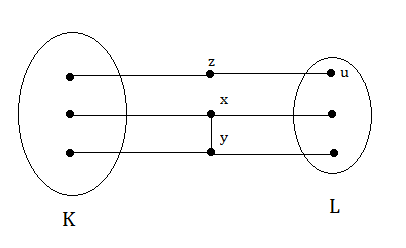
\includegraphics{img/kura1}
\caption{Componentes K y L en H}
\label{fig:kura1}
\end{figure}
La Figura 1 muestra distintos a los vecinos de $x, y, z$ en $K$ y $L$, pero esto podría no ser así. Lo que sí debe pasar es que deben tener vecinos tanto en $K$ como en $L$. Si alguno de los vértices $x$, $y$, $z$ no tuviera vertices adyacentes en $K$ o $L$, $H$ resultaría no conexo quitando solamente los otros dos vértices, lo cual es absurdo. Llamemos $u$ a un vértice adyacente a $z$, y consideremos la arista $a = \{z,u\}$. Contrayendo a $H$ por esa arista, por la hipótesis $C_a(H)$ no es 3-conexo, y por el mismo argumento por el que llegamos a que remover $\{x,y,z\}$ desconecta $H$, debe existir un vértice $v \in H$ tal que remover $\{z,u,v\}$ desconecta $H$. \\ \\
Sea $K'$ el subgrafo conexo inducido por los vértices de $K$, $x$ e $y$ (Figura 2) \\
\begin{figure}[htp]
\centering
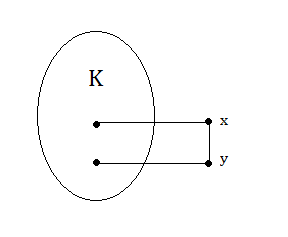
\includegraphics{img/kura2}
\caption{El subgrafo $K'$}
\label{fig:kura1}
\end{figure}
\newpage
Si el vértice $v$ estuviera entre los vértices de $K'$, entonces $K'\setminus\{v\}$ resulta conexo, pues de lo contrario $H\setminus\{z,v\}$ resultaría no conexo, absurdo por la 3-conexidad de $H$. Pero entonces $K'\setminus\{v\}$ es un subgrafo conexo de  $H\setminus\{x,y,z\}$ con más vértices que $K$ ($K'$ tiene dos vértices más que $K$ por tener a $x$ e $y$). Esto es absurdo, porque habíamos elegido $K$ maximal. \\\\ Entonces $v \notin V_{K'}$. Pero de esta manera alguna componente conexa de \newline $H\setminus\{z,u,v\}$ tiene a $K'$ como subgrafo, pero entonces $K$ no es maximal, absurdo. 
\end{proof}
\section*{Demostración del teorema}
\begin{definition}[Grafo de Kuratowki]
Se dice grafo de Kuratowski a todo grafo homeomorfo a $K_{3.3}$ o $K_5$
\end{definition}
\begin{lemma}
Una contracción no genera subgrafos homeomorfos a $K_{3.3}$ o $K_5$.
\end{lemma}
\begin{proof}[Demostración]
Supongamos que sí, es decir, existe un grafo $G$ que no tiene subgrafos de Kuratowski y posee una arista $e$ tal que $C_e(G)$ tiene un subgrafo de Kuratowski. Sea $K$ un subgrafo de Kuratowski en $C_e(G)$. $K$ debe contener al vértice $u$ generado en la contracción de $e = \{x, y\}$, de lo contrario $K$ sería un subgrafo de $G$, absurdo. $g(u)$ no puede ser 0 ni 1 en $K$, pues $K$ no sería homeomorfo a  $K_{3.3}$ o $K_5$.  Si $g(u) = 2$ en $K$, podemos obtener $K$ en $G$ reemplazando $u$ por $x$ o $y$ (Figura 3).\\ \\

\begin{figure}[htp]
\centering
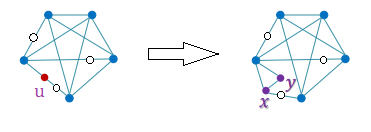
\includegraphics{img/kura5}
\caption{Si $u$ tiene grado 2 en $K$, podemos recuperar $K$ en $G$ (si hay mas vertices adyacentes a $x$ o $y$ son irrelevantes)}
\label{fig:kura1}
\end{figure}

Si $g(u) \ge 3$ en $K$ y solo $x$ (o solo $y$) es adyacente a 2 o mas vertices de $K$ en $G$, podemos tomar a $y$ (o $x$) como un vértice de subdivisión y conseguir un subgrafo de Kuratowski en $G$ (Figura 4). Absurdo, pues $G$ no tiene subgrafos de Kuratowski. \\

\begin{figure}[htp]
\centering
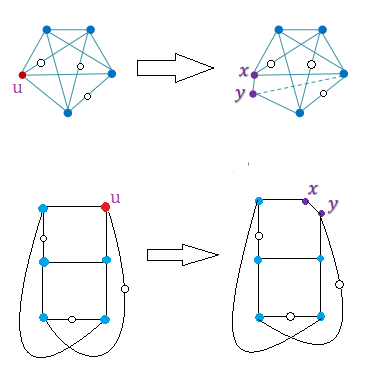
\includegraphics[width=7cm]{img/kura6}
\caption{Si solo $y$ o solo $x$ es adyacente a 2 o mas vertices de $K$ en $G$, podemos encontrar un subgrafo de Kuratowski en $G$}
\label{fig:kura6}
\end{figure}

El último caso es que $K$ sea homeomorfo a $K_5$ y que tanto $x$ como $y$ sean adyacentes a 3 de los vertices de $K$ en $G$. En ese caso existe un subgrafo homeomorfo a $K_{3,3}$ en $G$ (Figura 5), absurdo.


\begin{figure}[htp]
\centering
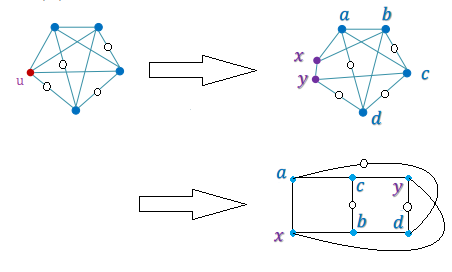
\includegraphics[width=7.5cm]{img/kura7}
\caption{Si tanto $x$ como $y$ son adyacentes a dos vertices de $K$ en $G$, podemos encontrar un subgrafo homeomorfo a $K_{3,3}$ en $G$.}
\label{fig:kura6}
\end{figure}
\end{proof}

\newpage
\begin{theorem}[Kuratowski]
Un grafo G es plano $\Leftrightarrow$ no tiene sugbrafos de Kuratowski
\end{theorem}
\begin{proof}[Demostración]
    ($\Longrightarrow$) Supongamos que existe G plano que contiene un subgrafo homeomorfo a $K_{3,3}$ o a $K_5$. Entonces existen inmersiones planas de esos subgrafos. Como las operaciones de homeomorfismo no alteran la planaridad del grafo (la remoción débil es una operación de contracción, que ya vimos que no afecta la planaridad, y la subdivisión elemental no puede generar un cruce de aristas en la inmersión plana), existe entonces una inmersion plana de $K_{3,3}$ o de $K_5$, absurdo pues no son planos (Lema 2).
\\\\
    ($\Longleftarrow$) Supongamos que existen grafos no planos que no son grafos de Kuratowski. Sea $G$ un grafo minimal (en cantidad de vértices y aristas) con esas características.
    Analicemos $K_v(G)$, la conexidad por vértices de G.\\\\
    Si $K_v(G) = 0$, el grafo no es conexo, luego existe una componente de $G$ con menos vértices que $G$, que no contiene subgrafos de Kuratowski. Absurdo pues $G$ es minimal.\\\\
    Si $K_v(G) = 1$, existe $v \in V_G$ vértice de corte. Existen $C_1, C_2, ..., C_k$ componentes conexas en $G\setminus\{v\}$, con $k \ge 2$. Sea $G_1$, el subgrafo inducido en $G$ por $V_{C_1} \cup \{v\}$, y $G_2$, el subgrafo inducido en $G$ por $V_{C_1} \cup V_{C_2} \cup ... \cup V_{C_k} \cup \{v\}$. \\
    Si $G_1$ o $G_2$ fueran no planos, deben tener un subgrafo de Kuratowski, pues tienen menos vértices que $G$, pero como son subgrafos de $G$, que no contiene subgrafos de Kuratowski, esto no puede ocurrir. Por lo tanto son planos, y por el Lema 1 existe una inmersión plana de cada uno que tiene a $v$ en la frontera de $R_\infty$. Entonces podemos construir a partir de ellas una inmersión plana de $G$, como muestra la Figura 3. Absurdo, pues $G$ no es plano. \\ 
\begin{figure}[htp]
\centering
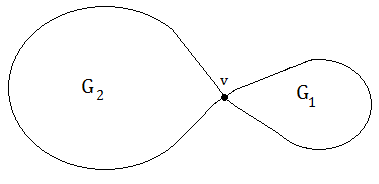
\includegraphics[width=7cm]{img/kura3}
\caption{Inmersión plana de $G$ a partir de las de $G_1$ y $G_2$}
\label{fig:kura1}
\end{figure} 
\\ \\
    Si $K_v(G) = 2$, sean $u$ y $v$ dos vértices que desconectan $G$. Existen $C_1, C_2, ..., C_k$ componentes conexas en $G\setminus\{u, v\}$, con $k \ge 2$. Sea $G_1$, el subgrafo inducido en $G$ por $V_{C_1} \cup \{u, v\}$, y $G_2$, el subgrafo inducido en $G$ por $V_{C_1} \cup V_{C_2} \cup ... \cup V_{C_k} \cup \{u, v\}$. \\ 
    Por un razonamiento análogo al anterior, $G_1$ y $G_2$ son planos, y por el Lema 1 existe para ambos una inmersión plana con la arista $e = \{u,v\}$ como frontera de $R_\infty$. Luego a partir de ellas se puede formar una inmersión plana de $G$, como ilustra la Figura 4. \\

\begin{figure}[htp]
\centering
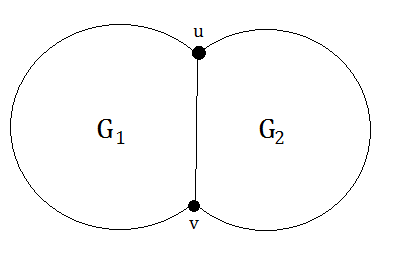
\includegraphics[width=7cm]{img/kura4}
\caption{Inmersión plana de $G$ a partir de las de $G_1$ y $G_2$}
\label{fig:kura1}
\end{figure}

Concluimos que $K_v(G) \ge 3$, luego $G$ es $3$-conexo. Al ser $3$-conexo, $G$ tiene al menos $4$ vértices, y $\forall v \in V_G, \ g(v) \ge 3 $. Pero el único grafo 3-conexo de $4$ vértices es $K_4$, un grafo plano. Por lo tanto $G$ tiene al menos $5$ vértices.  \\ \\
Por el Lema 3, entonces, existe $e \in E_G$ tal que $G' = C_e(G)$ es 3-conexo. Por el Lema 4 sabemos que $C_e(G)$ no contiene subgrafos de Kuratowski. y como tiene menos vértices que $G$, debe ser plano ($G$ es minimal). Sea $u$ el vértice formado en la contracción de $e$, y consideremos una inmersión plana de $C_e(G)$ que no tenga a $u$ en la frontera de la región externa (existe por el Lema 1). Si borramos todas las aristas que inciden en $u$, observamos que queda encerrado en un ciclo $C$ que contiene a todos los vértices adyacentes a $x$ o $y$ en $G$ (Figura 8). Etiquetamos $x_1, ..., x_r$ a los adyacentes a $x$: existen al menos dos de estos vértices, pues $g(x) \ge 3$ (el tercero es $y$). \\ \\
 \begin{figure}[htp]
\centering
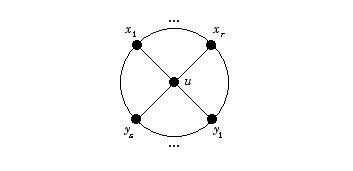
\includegraphics[width=7cm]{img/kura8}
\caption{Un ciclo $C$ encierra a $u$ en $C_e(G)$}
\label{fig:kura1}
\end{figure}

Analicemos lo que ocurre con los vértices adyacentes a $y$. Numeremolos $y_1, ..., y_s$ segun el orden en que aparecen en el ciclo en el sentido de las agujas del reloj. Si todos ellos se encuentran entre dos vértices $x_i$ consecutivos en el ciclo ($x_k$ y $x_{k+1}$ o $x_r$ y $x_1$, pudiendo coincidir en todo caso ${x_k} = y_n$ y $x_{k+1} = y_m$), existe una inmersión plana de $G$ colocando $x$ e $y$ en lugar de $u$ con sus aristas correspondientes (Figura 9)

 \begin{figure}[htp]
\centering
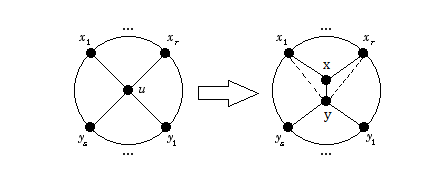
\includegraphics[width=10cm]{img/kura9}
\caption{Se logra una inmersion plana de $G$ si todos los $y_k$ están entre dos $x_i$ consecutivos (notese que $y$ puede ser adyacente a esos $x_i$ extremos).}
\label{fig:kura9}
\end{figure}

Si tres de los vertices adyacentes a $x$ lo son también a $y$ en $G$ (llamemoslos $a, b, c$, sea $K$ el subgrafo de $G$ formado por el ciclo $C$, los vértices $x$, $y$, la arista $\{x,y\}$ y las aristas que unen a $x$ e $y$ con $a$, $b$, y $c$. $K$ es homeomorfo a $K_5$ (Figura 10) y es un subgrafo de $G$, absurdo.

 \begin{figure}[htp]
\centering
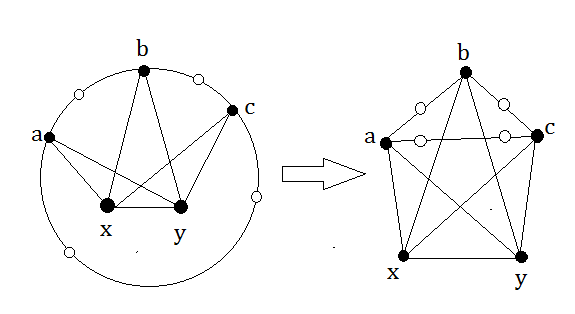
\includegraphics[width=9.5cm]{img/kura10}
\caption{Si tanto $x$ como $y$ son adyacentes a los mismos tres vertices del ciclo, existe $K$ subgrafo de Kuratowski en $G$.}
\label{fig:kura10}
\end{figure}


Por lo tanto no puede haber 3 vértices adyacentes a $x$ en $C$ que también lo sean a $y$ (caso 2), y no todos los adyacentes a $y$ pueden encontrarse entre dos adyacentes a $x$ consecutivos en el ciclo (caso 1). Entonces tenemos dos vértices $y'$, $y''$ adyacentes a $y$ y dos vértices $x'$, $x''$ adyacentes a $x$ que aparecen en el ciclo alternados en el orden $x', y', x'', y''$. Consideremos entonces el grafo $K$ formado por el ciclo $C$, los vértices $x$, $y$, la arista $\{x,y\}$ las aristas que unen a $x$ con $x', x''$ y a $y$ con $y', y''$. $K$ es un subgrafo de $G$, y es homeomorfo a $K_{3,3}$ (Figura 11), absurdo.
\begin{figure}[htp]
\centering

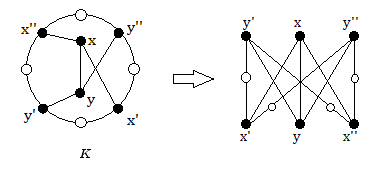
\includegraphics{img/kura11}
\caption{$K$ es homeomorfo a $K_{3,3}$}
\label{fig:kura11}
\end{figure}

En todos los casos llegamos a un absurdo. El absurdo viene de suponer que existe $G$, por lo tanto no puede existir, y entonces no existe ningún grafo no plano que no contenga un subgrafo de Kuratowski.

\end{proof}


\end{document}

